O objetivo final do projeto é caracterizar dimensões afetivas negativas em perfis do Twitter localizando pontos comuns entre usuários portadores de afetividades negativas (stress, ansiedade e depressão) de mesmo nível. Esse tipo de processo se assemelha com a aprendizagem não supervisionada, logo, antes dessa etapa é necessário mapearmos atributos, sendo assim, é necessário a identificação de usuários com dimensões afetivas negativas em primeiro momento.

Como observado, existem vários passos para conclusão desse projeto, abertamente estrutura de processamento contará com um processo de mineração e dois processos de inteligência artificial afim de gerar dois modelos lógicos. O objetivo dessa pesquisa é a primeira etapa do projeto, em outras palavras, o modelo responsável por inferir valores da EADS em um tweet.

Visando o objetivo inicial, é necessário fazer a máquina coletar e acertar as previsões com qualquer tipo de dado (mesmo que fornecido por pessoas não capacitadas, no caso uma base anotada pelo próprio autor), sendo assim, será detalhado o sistema em si (coleta de dados e aprendizagem de maquina) e as metodologias utilizadas para desenvolve-lo.

Pode-se observar na Figura \ref{fig:tecnologias}, o sistema é divido em dois núcleos, o Dumont responsável por minerar e gerar toda a base de dados, e o 14BIS que será responsável pelas inteligências artificias.

\begin{figure}
    \centering
    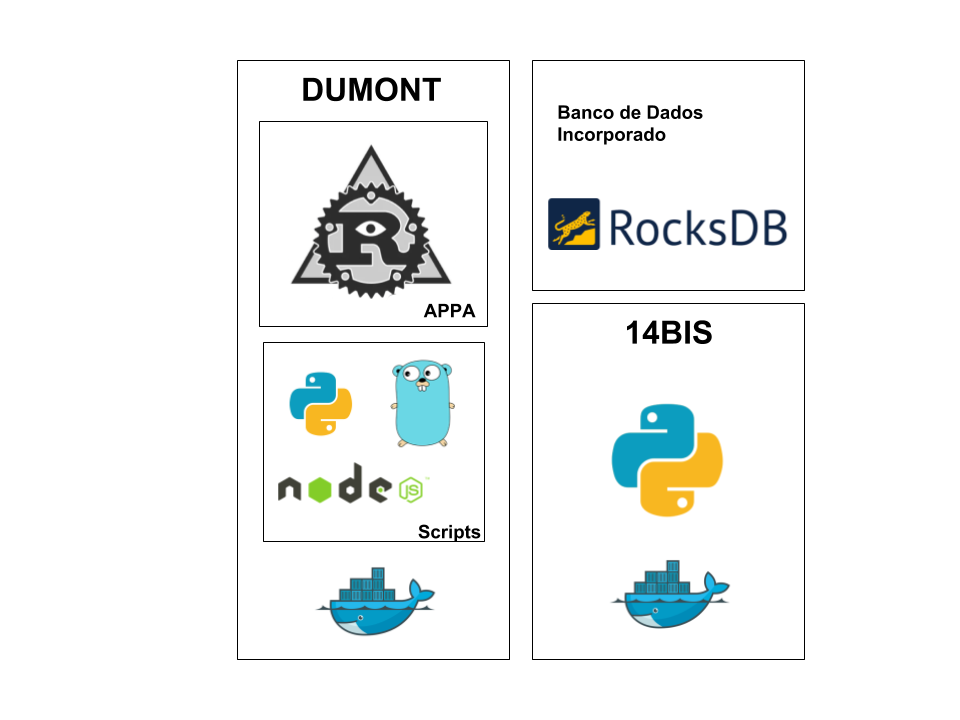
\includegraphics[width=0.9\textwidth]{imagens/tecnologias.png}
    \caption{Desenho apresentando os núcleos do projeto}
    \label{fig:tecnologias}
\end{figure}

Existem basicamente 5 tecnologias que estão sendo utilizadas nesse projeto:
\begin{itemize}
 \item Python: É a linguagem atual mais utilizada para o aprendizado de máquina, sua objetividade ja á torna simples de usar, porém, a quantidade de materiais, bibliotecas e artigos sobre PLN e Aprendizado de Máquina á tornam a principal linguagem nesse projeto.
 \item Node/Javascript: Node é o interpretador que permite com que seja possível executar o Javascript (linguagem originalmente de navegar no servidor). A linguagem tem um grande ganho com integrações e será utilizada para consumir recursos vindos de APIs.
 \item Go: Linguagem fortemente e estaticamente tipada, que fornecesse um poder de processamento equivalente a da linguagem C, entretanto, muito mais simples de escrever e manter código, será utilizado para scripts onde serão necessário processamento de muitos dados.
 \item MongoDB: O Mongo é um banco não relacional, que guarda dados em formato de documentos, muito utilizado no mercado recentemente.
 \item Docker: Docker é uma ferramenta para infraestrutura, será utilizado para rodar a aplicação em containers e facilitar o \textit{deploy}\footnote{Vindo do termo em inglês "lançar" é utilizado para o ato de colocar uma aplicação em ambiente de produção}.
\end{itemize}

Todo o código dos núcleos previamente demonstrados está disponível no GitHub. Para entender como funciona a plataforma de versionamento, que pode ser também utilizada para achar informações mais técnicas além de baixar o código basta seguir as instruções conforme o \autoref{app:git}. Além disso como mostrado ambos os núcleos utilizam Docker como base para executar as aplicações, isso devido ao resultado de tal abordagem reduzir alguns problemas possíveis em relação a ambiente de execução. É possível obter as informações necessárias para entendimento e instalação conforme o \autoref{app:docker}.

Uma vez obtido conhecimento sobre os núcleos do projeto e suas tecnologias, é possível idealizar o fluxo completo e interação entre elas. Se observar a Figura \ref{fig:tcc_caso_de_uso}, notara que o Dumont ira utilizar da API do Twitter para coletar dados públicos, posteriormente esses dados serão processados e mutacionados a fim de gerar uma base de dados, por final essa base dados será salva em um banco de dados.

\begin{figure}[!h]
    \centering
    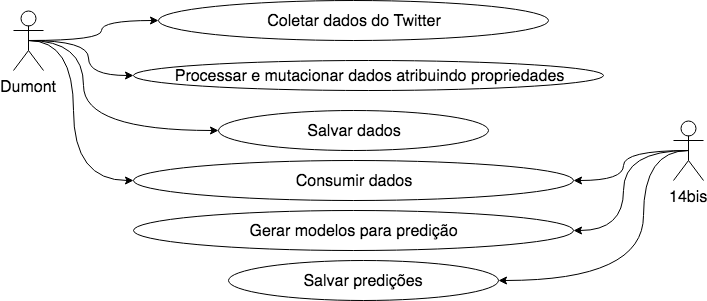
\includegraphics[width=.5\textwidth]{imagens/tcc_caso_de_uso.png}
    \caption{Diagrama de caso de uso do sistema}
    \label{fig:tcc_caso_de_uso}
\end{figure}

Para salvar os dados durante a coleta ou o pré-processamento será utilizado o MongoDB. O MongoDB  é um banco não relacional, ou seja, um banco que não tem \textit{transactions}\footnote{Simboliza uma atividade realizada em um banco relacional} e é baseado inteiramente em documentos. Diferente de um banco não relacional, os dados inseridos nesse tipo de banco não têm uma normalização ou qualquer tipo de padrão. No caso do Mongo a única identificação utilizada para interligar os documentos é a nomeada coleção\footnote{As Coleções servem para agrupar tipos especificos de documentos.}.

Dentro do trabalho existem algumas estruturas mais fechadas e outras que irão variar mais com o passar do desenvolvimento, pode-se notar na Figura \ref{fig:entities}, a visão inicial do que seria a estrutura de nossos documentos. Teremos duas coleções mais relevantes \textit{Tweet} e \textit{User} aqui ficaram armazenados os dados do Twitter, as demais estruturas são estruturas periféricas criadas para suportar o sistema de armazenamento de dados especialistas. Para isso existe a estrutura \textit{Answer} que serve para que os especialistas inserirem a possibilidade de um mapeamento de algum dos items da EADS para um tweet. Por final existem mais duas coleções a \textit{Specialist} que armazena os especialistas registrados no nosso sistema e o \textit{List} que é uma coleção auxiliar para agrupar uma quantidade de tweets tornando mais fácil para nossa aplicação apresenta-los aos especialista e coletar analise.

\begin{figure}[!h]
    \centering
    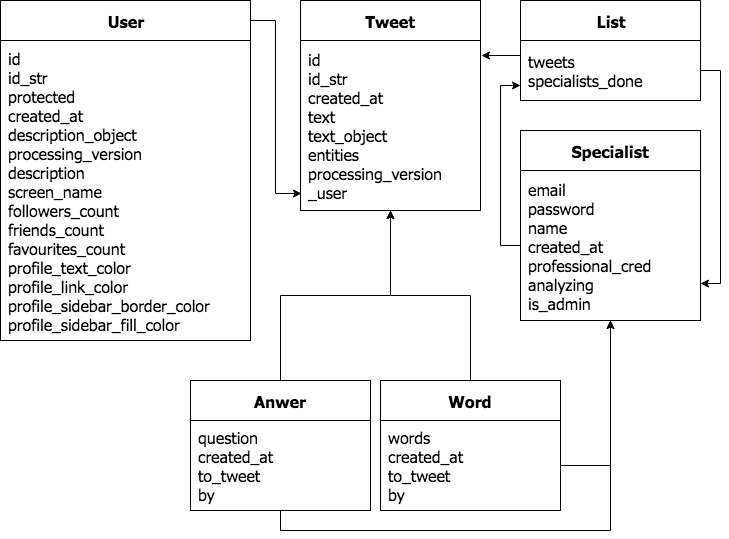
\includegraphics[width=.65\textwidth]{imagens/entities.png}
    \caption{Mapa de entidades do projeto}
    \label{fig:entities}
\end{figure}

Vale ressaltar que o objetivo é gerar uma base de conhecimento, e isso implica na ausência de profissionais agindo na base nesse primeiro trabalho. Além disso aplica-la a uma aprendizagem supervisionada e em seguida aplicar esse dado a uma não supervisionada. Logo a primeira etapa é adquirir o \textit{dataset} que será utilizado.

\section{Coletando Base de Dados}
A primeira etapa do processo inclui coletar dados para que, posteriormente, seja possível mineirar atributos dentro deles. O coletor é algo simples, basicamente um script que roda de tempos em tempos baseado na configuração apresentada. Foi desenvolvida uma função responsável por coletar em tempo real tweets em uma determinada área e que em seu corpo tivesse uma ou mais palavras chaves. Com isso é possível pesquisar um usuário e seus últimos 200 tweets.

De todos os modelos previamente explicados, os utilizados dentro do coletor são os de \textit{user} e \textit{tweet}. Eles podem ser encontrados dentro de \textit{dumont/collector/schemas}. Antes do dado ser salvo é possível notar a criação de um objeto partindo do atributo de texto referente ao tweet. Um dos problemas durante a mineração de dados é o uso de \textit{emojis} em textos. Sabendo que \textit{emojis} podem expressar sentimentos, armazenar e tratar esses dados poderia ser relevante na hora de confirmar o sentimento em frases, durante esse processo a lógica para localizar e extrair esses elementos foi abstraida para uma biblioteca chamada \textit{Emojinator}\footnote{https://github.com/getdumont/emojinator}. Além do texto tratado, também será obtida informações do \textit{emojis} utilizados no meio do texto.

Para ativar o coletor foi criado um CLI\footnote{CLI é abreviatura para \textit{Command Line Interface}, em outras palavras, uma interface que permite executar códigos direto do terminal}. Antes de rodar o comando é necessário configurar o projeto conforme o \autoref{app:configuracoes}. Após terminar a configuração rode o comando \textit{docker-compose up collector}, logo que finalizar a coleta vai preencher seu MongoDB com os dados necessários para as próximas etapas. Durante essa pesquisa o comando foi rodado diversas vezes em um periodo de tempo, para criar uma base inicial. Vale lembrar que a idéia final se consiste em um mapeando periódico de perfis, porém nesse momento o coletor foi feito unicamente para juntar um aglomerado de dados indiferente de seus perfis.

No primeiro momento que o coletor foi rodado na pesquisa, foram coletados um total de 68583 tweets distribuídos entre 419 perfis, gerando uma média de aproximadamente 163 tweets por usuário. A massa de dados é bem ampla e achar uma amostra que suprisse as necessidades poderia ser algo complexo. Para isso o enfoque inicial é localizar uma amostra com os perfis que contem a maior massa de tweets negativos, entretanto, isso não é possível sem idealizar uma segunda parte do processo, no caso o pré-processamento e a mineração.

\subsection{Tarefas de Pré-Processamento}
O segundo passo após coletar os dados é rodar scripts de pré-processamento e mineração. Uma das maiores dificuldades é como manipular os dados de maneira incremental. Desde que a pesquisa teve inicio, muitas idéias surgiram, novos pontos de vistas e novos dados a serem minerados. Foi adotado uma propriedade chamada \textit{processing\_version}, essa propriedade marca o documento com a versão do processamento dele.

Dentro da pasta \textit{dumont/tasks/processing} existem duas pastas, com código para processar usuários e outra para processar tweets, ambas contem vários estágios de processamento, esses são exportados e passados para uma classe chamada \textit{Processor} localizada no arquivo \textit{dumont/tasks/processing/\_\_init\_\_.py}, o nível de processamento base é o 0 (nível inserido na hora que o coletor salva do dado no banco), a partir disso é possível atualizar o processamento por um script.

As tarefas de processamento são responsáveis por:

\begin{itemize}
    \item Normalização de Palavras: Transformar girias e erros conhecidos em palavras corretas.
    \item Remoção de \textit{stop-words}: Existem palavras que prejudicam a analise textual por não serem essenciais ou estarem colocadas de maneira equivocada. Um dos processos retira esse tipo de ruído do texto.
    \item Arvore Léxica: Criar uma arvore léxica baseada na frase original do tweet e na frase que já foi tratada removendo as \textit{stop-words}.
    \item Analise de Sentimento: Utilizando a API do Google Language é retirado o sentimento da frase original e da frase tratada também.
\end{itemize}

As tarefas sofreram aprimoramento durante a analise de dados, entretanto, o que será exposto aqui é o estagio de refinamento obtido até o momento junto com seus resultados. Enquanto a análise era feita foi notado uma quantidade de girias e expressões que podiam influenciar a analise de sentimento, tão quanto a extração de arvore lexica. Fazendo assim com que dois dos principais atributos a serem mapeados ficassem inconsistentes. Conforme \ref{app:tabelanorm} que traz uma tabela com termos, é possivel notar todas as palavras, as substituições e a quantidade encontrada no banco inicial.

Além disso, foi encontrado um outro padrão devido a uma recente moda chamada CuriousCat\footnote{\url{https://curiouscat.me}}, um site de perguntas e respostas. Muitos tweets contem textos referentes a função de compartilhamento da plataforma. Algumas respostas podem ajudar na inferencia, logo foi criado um script para substituir o tweet, usualmente formado pela pergunta juntamente com uma parte da resposta, por unicamente a resposta completa(indiferente do seu tamanho), para isso foi criado um \textit{WebScraping}\footnote{termo utilizado para \textit{scripts} que "raspam" ou coletão dados de páginas da web através de API ou de algoritimos de automação que buscam valores em telas HTML} que pode ser encontra no arquivo \textit{dumont/tasks/processing/entity\_parser/url/curiouscat.py}\footnote{Código fonte no GitHub: \url{}}.

Um outro grande problema apresentado durante a analise é que muitos tweets expressavam sentimentos, porém seu discurso era dividido, ou seja, o texto em si representava apenas uma parte do conteúdo da publicação. No caso existem tweets unicamente com imagem e casos onde o texto é uma mera legenda para a imagem, além disso existem publicações com vídeos e publicações divididas em vários tweets, ou seja, expressões como \textit{emojis}, risadas e outras ferramentas dissertativas que não trazem diretamente um conteudo e sim um apoio a um ou mais tweets anterioriores. Entretanto tratar isso levaria tempo, então nesse primeiro passo da pesquisa esses dados foram ignorados.

Todas as alterações geram novos atributos, principalmente o \textit{clean\_text} que servira como base para retirada de informações, para executar o \textit{script} necessário para essa ação basta rodar o comando \textit{docker-compose up tasks}. Com esses dados já é possível ter alguma noção de informações relevantes dos textos, porém ainda é necessário de embasamento técnico, ou seja, um dado especialista que possa orientar a máquina a utilizar as demais propriedades mapeadas para localizar um delta em comum, entretanto, exigir que todos os dados da massa sejam analisados é algo inviavel. Para isso é necessário gerar uma pré-amostra.
\section{Amostras e Análise de Dados}
Com os textos devidamente pré-processados e com os atributos selecionados, é necessário a coleta de uma amostra para que seja possível em uma segunda parte do processo, adicionar os atributos referentes a futura inferência da EADS, para que essa amostra seja coletada é necessário que em primeiro instante seja feita uma análise dos dados. Para entender a próxima análise é necessário compreender que a análise de sentimento retorna dois fatores: score e magnitude, o score varia entre 1 e -1, sendo 1 representativo ao sentimento positivo e -1 o negativo, logo 0 seria neutro. Além disso existe a magnitude que é para expressar o quão o sentimento é presente no texto. 

No caso do Twitter (280 caracteres máximos) por postagem as pessoas tendem a ser mais diretas e sucintas, logo a magnitude é muito variável e pode ser um dado que venha a confundir em vez de ajudar, logo, foi agrupado os tweets pelos scores, a cada espaçamento de 0.2. Ao observar o Figura \ref{fig:sentiment-relation}, notasse que as extremidades tendem a ter menos tweets, média de 1000 a 2500 tweets por agrupamento, entretanto grupos mais centralizados (emoções neutras) chegam a picos de 8104 tweets, já que o dado desejado é uma massa negativa e seus usuários será dado enfoque ao lado negativo do mapeamento.

\begin{figure}
    \centering
    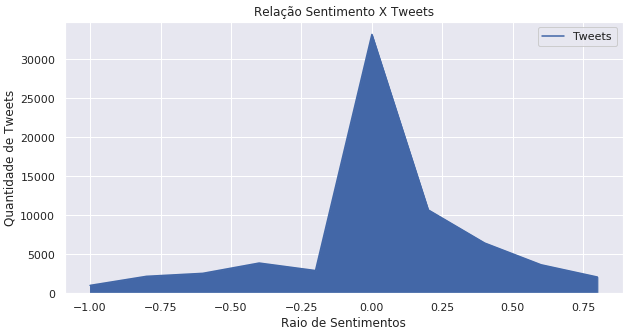
\includegraphics[width=.4\textwidth]{imagens/relacao-sentimento.png}
    \caption{Relação de sentimentos por tweet dentro da massa de dados}
    \label{fig:sentiment-relation}
\end{figure}


Partindo do principio que a partir de um score de -0.2 já existem menos dados, foi tomada como premissa que qualquer dado com score superior a esse é um dado não viável para amostra. Seguindo essa premissa é preciso mapear de cada usuário o percentual de publicações a abaixo de -0.2, com isso será possível obter um percentual da densidade de publicações negativas naquele perfil. Analisando os dados da Figura \ref{fig:negative-pop-relation}, é possível notar que a maior quantidade de percentual negativo esta entre 20\% e 40\%, entretanto, é impossível afirmar que os dados suprem as necessidades que a inteligência artificial ira necessitar para realizar a inferência na base. Refletindo sobre a EADS, a versão minificada tem 21 perguntas, logo, necessita-se de no mínimo 21 tweets negativos na esperança que cada um responda pelo menos 1 das perguntas. Para validar a ideia é necessário descobrir a média de tweets dentro dos percentuais que mais contem massa negativa.

\begin{figure}[!h]
    \centering
    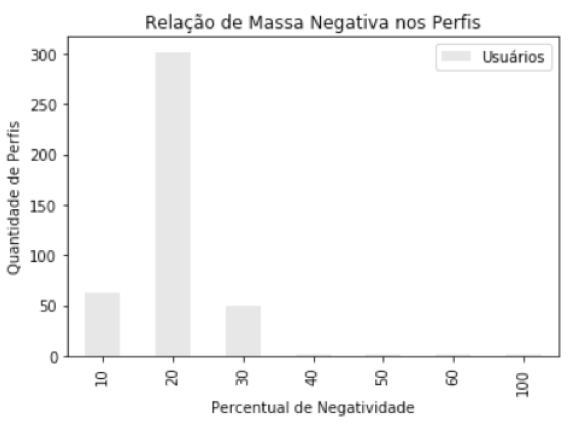
\includegraphics[width=.4\textwidth]{imagens/relacao-massa-neg.png}
    \caption{Percentual de massa negativa por quantidade de perfis}
    \label{fig:negative-pop-relation}
\end{figure}

Entretanto, pode-se notar mais um fator no dado, existem perfis com 100\% de sentimento negativo devido a conter um único tweet negativo, ou seja, a quantidade de tweets é algo relevante. Logo foi feito uma cáculo a partir dos dados retirados, a quantidade de tweets negativos entre 20\% a 40\% de massa negativa é equivalente a 9592, de um total de 413 usuários, a média retirada foi de aproximadamente 23 tweets negativos por usuário da massa.

Uma vez obtido os dados do percentual e média de tweets é possível configurar o script para gerar amostra. Como dito são 21 questões, que representam o total de questões da EADS, logo, é necessário um mínimo de 21 tweets negativos (já contemplado pela média de 23), logo para aumentar a eficácia uma nova média foi retirada do dobro de questões somado a média atual de tweets negativos, o que deu aproximadamente 32 tweets. Dessa amostra foram minerados 21 perfis e 907 tweets negativos. Se observar as Figura \ref{fig:sample-relation} é possível notar que a média de tweets negativos pegos para análise em relação a base é de 1.3\% enquanto em relação aos usuários 5\%.

\begin{figure}[!h]
    \centering
    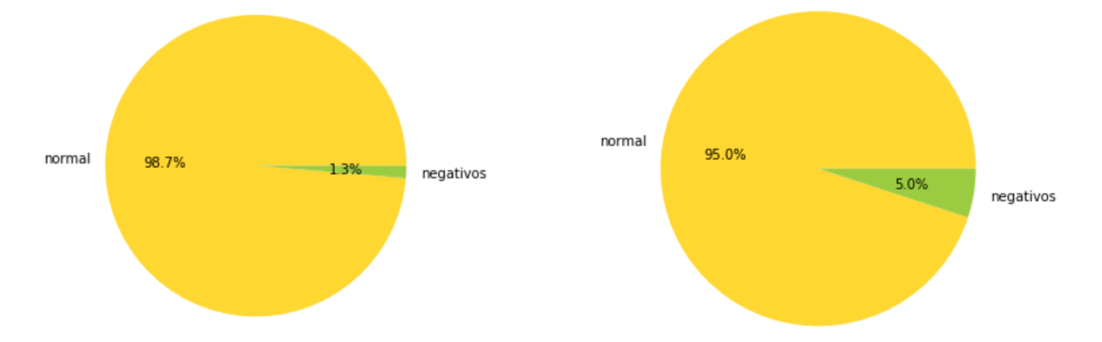
\includegraphics[width=.6\textwidth]{imagens/relacao-amostra.png}
    \caption{Percentual de dados utilizados na amostra em relação a base total de tweets e usuários}
    \label{fig:sample-relation}
\end{figure}


\section{Dados Especialistas}
Para facilitar a inserção de dados especialistas foi criado uma interface para mapear possíveis questões da EADS nos tweets. Para ativar a plataforma de inserção de dados especialistas basta utilizar o comando \textit{docker-compose up specialist\_app}, caso deseje subir essa aplicação online será necessário um serviço de núvem, porém, a aplicação rodada local pode ser acessada para \textit{\url{http://localhost:3000}}.

Os dados foram inseridos manualmente simulando especialistas, sem lógica de ponderação. Todos os dados que serão apresentados foram anotados pelo autor e não por especialistas. A partir disso foram encontrados na analise 312 tweets com perguntas inseridas, entretanto, um tweet pode responder mais de uma pergunta, foram inseridas um total de 688 perguntas. Como apresentado na Figura \ref{fig:question-balance} e conforme o \ref{app:eads} é possível ver que as questões que mais contém respostas são questões mais voltadas a situação psicológica, sendo mais frequente expressa-las involuntáriamente durante seu discurso. Em contra partida as perguntas com menos respostas são questões referentes a situações fisicas.

\begin{figure}[!ht]
    \centering
    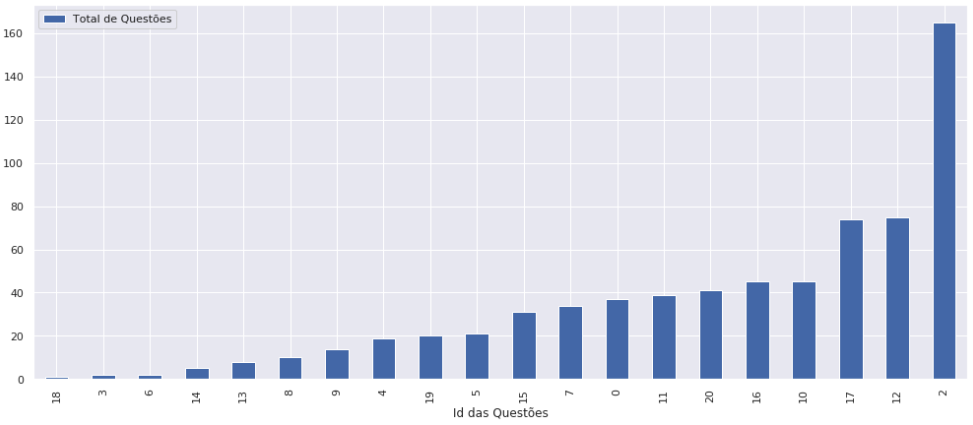
\includegraphics[width=.55\textwidth]{imagens/question-balance.png}
    \caption{Relação de Perguntas Respondidas por Tweets}
    \label{fig:question-balance}
\end{figure}

As questões com menor resposta estão atreladas com ansiedade conforme \ref{app:eads}, isso afeta o desempenho do projeto final, entretanto, é possível encontrar relações e aproximar os valores para chegar no resultado final. Em primeiro momento o objetivo é apenas inferir perguntas (ignorando até mesmo o impacto), já que não existem informações suficientes relacionadas a essas questões a máquina não conseguira inferir essa informação, entretanto, não irá impedir que as demais perguntas sejam devidamente inferidas.


